% -----------------------------------------------------------------------------
% Artigo — Aprendizado de Máquina II (PUC Minas, 2026/2)
% Formatado no padrão SBC (sbc-template.sty). No Overleaf, use o modelo
% "SBC Conferences Template" ou mantenha o sbc-template.sty no mesmo projeto.
% Arquivos do projeto: referencias.bib, figuras/ (PDFs), tabelas/ (.tex).
% Compilador: pdfLaTeX.
% -----------------------------------------------------------------------------
\documentclass[12pt]{article}
\usepackage{sbc-template}
\usepackage{graphicx,url}
\usepackage[utf8]{inputenc}
\usepackage[brazil]{babel}
\usepackage[T1]{fontenc}
\usepackage{lmodern}
\usepackage{amsmath,amssymb}
\usepackage{booktabs,tabularx,multirow}
\usepackage{xcolor}
\sloppy

\newcommand{\repo}{\textcolor{red}{[https://github.com/paraenseembh/ap2\_perfis1\_de\_cartoes]}}\renewcommand{\tabularxcolumn}[1]{m{#1}}
\newcolumntype{L}{>{\raggedright\arraybackslash}X}
\newcolumntype{P}[1]{>{\raggedright\arraybackslash}p{#1}}
\makeatletter\newcommand{\tabinput}[1]{\@@input #1 }\makeatother

\title{Detectando o anômalo pelo perfil: introdução ao aprendizado não supervisionado com dados de compra sem rótulos}

\author{Lucas Rafael Nascimento\inst{1}, Maria Vitoria Manhães\inst{1},\\
  Rafael Cabral\inst{1}, Tainara Almeida\inst{1}}

\address{
Bacharelado em Ciência de Dados e Inteligência Artificial\\
Pontifícia Universidade Católica de Minas Gerais (PUC Minas)\\
Belo Horizonte, MG -- Brasil\\
Repositório: \repo
}

\begin{document}
\maketitle

\begin{resumo}
Em uma operadora de pagamentos simulada, analisamos 3.000 perfis de clientes sem rótulos, com o propósito de segmentar o consumo e priorizar clientes suspeitos de fraude. K-Means, GMM e HDBSCAN recuperaram a mesma partição em quatro perfis, e a diferença entre eles está no score de anomalia. Defendemos que a fraude deve ser modelada como desvio em relação ao perfil do próprio cliente, e não como valor extremo. Entre os scores avaliados, o GMM, com frequência desquantizada e score $-\log p(x)$ médio, foi o mais estável (Jaccard de 0,664 em execução única e de 0,967 em ensemble).

\textbf{Palavras-chave}: detecção de fraudes; aprendizado não supervisionado; GMM; segmentação de clientes; score de anomalia.
\end{resumo}

\begin{abstract}
We analyse 3,000 unlabelled customer profiles from a simulated payment operator, segmenting consumption and ranking suspicious customers. K-Means, GMM and HDBSCAN recover the same four segments, and they differ only in their anomaly scores. We argue that fraud should be modelled as a deviation from each customer's own profile rather than as an extreme value. Among the scores evaluated, the negative log-likelihood of a GMM fitted on dequantised data, averaged over several dequantisations, proved the most stable.

\textbf{Keywords}: fraud detection; unsupervised learning; GMM; customer segmentation; anomaly score.
\end{abstract}

% =============================================================================
\section{Introdução}
Fraudes bancárias digitais e golpes com cartões somaram R\$~10,1 bilhões em perdas no Brasil em
2024, segundo a Febraban \cite{febraban2025}, e o uso indevido de cartão por terceiros continua
entre os tipos de fraude mais relatados pelos consumidores \cite{serasa2025}. Diante desse cenário,
a detecção automatizada esbarra em uma limitação estrutural: rótulos confiáveis de fraude são
escassos, chegam com atraso e cobrem apenas os padrões já conhecidos. Métodos não supervisionados
surgem, então, como uma forma de atribuir \emph{scores de suspeita} que orientam a investigação
humana, sem a pretensão de comprovar a fraude \cite{bolton2002fraud}.

Este trabalho examina uma base exclusiva e sem rótulos, proveniente de uma operadora de pagamentos
simulada, com dois objetivos: segmentar os clientes em perfis de consumo e identificar aqueles cujo
comportamento é atípico o bastante para justificar revisão. A pergunta que orienta o artigo é qual
dos algoritmos vistos na disciplina constitui a melhor escolha \emph{para esta base}, e não em geral.

Nossa resposta tem duas partes. Quando os dados descrevem perfis agregados bem separados, a escolha
do algoritmo de segmentação deixa de ser decisiva, porque métodos de naturezas diferentes convergem
para a mesma partição, e a decisão relevante passa a ser \emph{como medir o desvio}. Defendemos que a
fraude deve ser tratada como desvio contextual, isto é, em relação ao perfil do próprio cliente, e que
o GMM é a escolha mais adequada, pois entrega, em um só modelo, a segmentação e um score probabilístico
contextual, estável e acompanhado de um critério próprio para escolher $K$.

O trabalho traz quatro contribuições. A primeira é um diagnóstico da base, que mostra a redundância
exata entre atributos e o efeito da frequência discreta sobre o BIC e o HDBSCAN. A segunda é uma
comparação entre K-Means, GMM, DBSCAN e HDBSCAN quanto à qualidade interna, à estabilidade da partição
e à estabilidade do score de anomalia. A terceira é um protocolo de score médio sobre várias
desquantizações, que torna reprodutível o ranking de suspeitos. A quarta consiste em recomendações
operacionais com limiares por perfil.

% =============================================================================
\section{Fundamentação Teórica}
\subsection{Tipos de fraude bancária}
Organizamos as fraudes pelo \emph{mecanismo}, já que ele determina o que um dado agregado consegue
revelar (Tabela~\ref{tab:fraudes}). Nas fraudes com cartão (clonagem, uso sem a presença física, troca
de cartão e \emph{card testing}), o titular não participa da transação. Na \emph{tomada de conta}
(\emph{account takeover}), o criminoso opera a conta com credenciais roubadas. Na fraude de
\emph{identidade}, contas são abertas com documentos roubados ou sintéticos e, com frequência, viram
contas ``laranja''. Na \emph{engenharia social}, é a própria vítima que autoriza o pagamento, como nos
casos de falsa central, falso parente ou falsa venda. Por fim, na fraude de \emph{primeira parte}, o
próprio cliente frauda, seja no \emph{bust-out}, em que ele constrói histórico e esgota o limite, seja
na contestação indevida de compras legítimas.

\begin{table*}[t]
\centering\small
\caption{Tipos de fraude, sinal esperado em dados agregados de frequência e ticket por cliente, e
observabilidade nesta base (sem dimensão temporal, de estabelecimento ou de localização).}
\label{tab:fraudes}
\begin{tabularx}{\textwidth}{@{}P{3.1cm}L L P{2.3cm}@{}}
\toprule
\textbf{Tipo} & \textbf{Mecanismo} & \textbf{Sinal esperado no perfil agregado} & \textbf{Observável aqui?} \\
\midrule
Cartão: \emph{card testing} / cartão não presente & Dados vazados testados com compras pequenas e repetidas & Frequência alta com ticket atipicamente baixo para o perfil & Sim (contextual) \\
Cartão: clonagem / troca & Cartão copiado ou trocado é usado por terceiros & Poucas compras de valor alto & Parcial \\
Tomada de conta & Credenciais roubadas; uso como se fosse o titular & Ruptura em relação ao histórico do próprio cliente & Não (exige tempo) \\
Identidade / contas laranja & Abertura com dados falsos; contas para escoar valores & Contas em lote com comportamento idêntico & Parcial (anomalia coletiva) \\
Engenharia social & A vítima autoriza a transação & Indistinguível do comportamento legítimo & Não \\
Primeira parte (\emph{bust-out}) & O cliente esgota o limite sem intenção de pagar & Poucas compras, ticket muito acima do perfil & Parcial \\
\bottomrule
\end{tabularx}
\end{table*}

\subsection{Perfis de consumo e perfis atípicos}
Frequência e valor monetário são dois dos três eixos clássicos do modelo RFM (recência, frequência e
valor), no qual o valor monetário corresponde ao gasto médio por transação \cite{fader2005rfm}. A base
deste trabalho contempla os eixos F e M, mas não a recência. A segmentação de mercado por agrupamento é
tradicional em marketing, e os modelos de mistura finita figuram entre suas vertentes metodológicas
centrais \cite{wedel2000segmentation}. No Brasil, a combinação entre RFM e K-Means já foi empregada em
estudos com dados de e-commerce \cite{kutz2025rfm} e de varejo de vestuário \cite{fernandes2022rfm}.

Neste trabalho, distinguimos três tipos de perfil atípico: o \emph{global}, que está longe de todos os
perfis; o \emph{contextual}, que está dentro de um perfil, mas na sua borda; e o \emph{coletivo}, em que
um grupo se comporta de maneira estranha como conjunto. Comparar um cliente com seus pares, e não com a
população inteira, é a base da \emph{peer group analysis} aplicada à fraude em cartões
\cite{weston2008peer}. Ainda assim, atípico não equivale a fraudulento: a análise estatística produz
suspeita, e não prova \cite{bolton2002fraud}.

% =============================================================================
\section{Trabalhos Relacionados}
O GMM já foi empregado como componente não supervisionado em um pipeline híbrido de detecção de fraude
em cartões \cite{silva2025gmm}. Outro estudo comparou algoritmos de agrupamento e de detecção de outliers
sobre transações categorizadas, valendo-se de métricas internas de validação \cite{oliveira2023spending}.
A combinação de detectores de anomalia com análise visual, com o objetivo de reduzir falsos positivos,
aparece em \cite{torres2020visual}. Para contornar a escassez de dados públicos, um simulador de
transações sintéticas foi construído \cite{santos2024sintetico}. Em escala internacional, aprendizado
não supervisionado foi aplicado a transações de um banco grego \cite{karnavou2025fraud}.

% =============================================================================
\section{Base de Dados e Pré-processamento}
\label{sec:eda}
A base contém 3.000 clientes descritos por quatro colunas: \texttt{id\_cliente},
\texttt{valor\_total\_gasto}, \texttt{frequencia\_compras} e \texttt{ticket\_medio}. Não há valores
ausentes, identificadores repetidos, variáveis categóricas ou componentes temporais. Há, no entanto, 51
clientes, distribuídos em 25 grupos, com valores idênticos nas três variáveis, ainda que com
identificadores distintos. Esses registros foram mantidos e tratados como possível anomalia coletiva.

Há também uma redundância exata entre os atributos. O ticket médio coincide com
$\text{valor}/\text{frequência}$, com erro máximo de 0,005 que se deve apenas ao arredondamento. Em
escala logarítmica, a relação torna-se linear e exata, o que a PCA sobre as três variáveis em log
confirma: os componentes explicam 68,9\%, 31,1\% e 0,0\% da variância. Por isso, mantivemos apenas
frequência e ticket. O valor total ficou fora da modelagem para não pesar duas vezes na distância e foi
usado apenas na interpretação.

A distribuição das variáveis também merece atenção. O valor total tem cauda longa, com assimetria de
1,69 que cai para 0,12 após o log. A frequência e o ticket, por sua vez, são bimodais e formam quatro
blocos visíveis (Figura~\ref{fig:estrutura}), separados por vazios quase completos: apenas 1 cliente tem
entre 8 e 24 compras, e somente 6 têm ticket entre R\$~60 e R\$~220. Esses 7 clientes são, portanto, os
candidatos naturais a anomalia \emph{global}. Frequência e ticket, por outro lado, são praticamente não
correlacionados (Spearman de 0,028).

\begin{figure}[t]
\centering
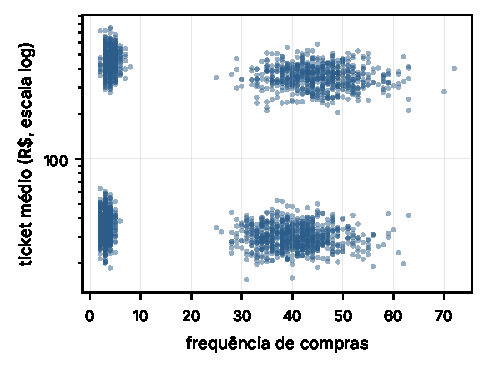
\includegraphics[width=\columnwidth]{figuras/f1_estrutura.pdf}
\caption{Frequência $\times$ ticket médio (escala log). Os quatro blocos são separados por vazios.}
\label{fig:estrutura}
\end{figure}

Os critérios univariados tradicionais também enganam. Na escala bruta, o critério IQR marca 609 clientes
em valor total, e o z-score robusto (MAD, com limiar de 3,5) marca 1.358 em frequência. Em log, nenhum
dos dois critérios marca clientes nessas variáveis. Os ``outliers'' da escala bruta são, portanto, um
efeito da bimodalidade, e não clientes estranhos, razão pela qual nenhum ponto foi removido: em fraude,
o valor extremo pode ser justamente o sinal que se procura.

A frequência, por sua vez, assume apenas 47 valores inteiros e, em escala logarítmica, a distância entre
2 e 3 compras é grande, o que cria ``degraus'' artificiais de densidade. Para atenuar esse efeito,
aplicamos uma \emph{desquantização}: somamos à contagem, antes do logaritmo, um ruído
$U(-0{,}5;\,0{,}5)$, procedimento usual na modelagem de densidades sobre dados discretos
\cite{theis2016dequant}. Trata-se de uma decisão heurística, cujo efeito é avaliado na
Seção~\ref{sec:res}. Com isso, o espaço final é $\mathbf{x}=(\log \tilde f,\ \log t)$, padronizado com
\texttt{StandardScaler}, em que $\tilde f$ denota a frequência desquantizada e $t$ o ticket médio.

Esse diagnóstico restringe a escolha dos algoritmos. Os grupos são compactos e bem separados, o que tende a
facilitar a segmentação. Em contrapartida, quase não há pontos fora dos blocos (apenas 7 em 3.000), de
modo que a anomalia possível é, em sua maior parte, \emph{contextual}. A densidade também varia entre os
blocos, o que desafia parâmetros globais como o $\varepsilon$ do DBSCAN, e a frequência discreta pode
inflar o número de grupos escolhido por critérios de densidade. Por fim, com apenas duas dimensões
efetivas, t-SNE e UMAP tornam-se desnecessários para a visualização.

% =============================================================================
\section{Metodologia}
Escolhemos quatro abordagens de naturezas distintas, resumidas na Tabela~\ref{tab:algos}: o K-Means
\cite{macqueen1967kmeans}, de caráter particional; o GMM ajustado por EM \cite{dempster1977em}, de
caráter probabilístico; e o DBSCAN \cite{ester1996dbscan} e o HDBSCAN \cite{campello2013hdbscan}, ambos
baseados em densidade. Além delas, incluímos a densidade por kernel (KDE), função sobre a qual o DENCLUE
sobe até os atratores \cite{hinneburg1998denclue}, que serve como score de comparação. Outras alternativas
foram descartadas por razões específicas à base. O AGNES equivale ao K-Means nesta base e tem custo
$O(n^2)$; o BIRCH só se justifica em grandes volumes; o ROCK foi concebido para dados categóricos; o SOM é
desnecessário, já que os dados são bidimensionais; a biclusterização não se aplica a apenas dois atributos;
e o K-Medoides perde sentido porque, em log, não há outliers que distorçam os centroides. Isolation Forest e
LOF não fazem parte do conteúdo da disciplina e ficaram como trabalho futuro.

\begin{table*}[t]
\centering\small
\caption{Premissas de cada algoritmo $\times$ evidência da análise exploratória.}
\label{tab:algos}
\begin{tabularx}{\textwidth}{@{}P{1.7cm}L L L P{2.6cm}@{}}
\toprule
\textbf{Método} & \textbf{Premissa} & \textbf{Evidência a favor} & \textbf{Evidência contra / limitação} & \textbf{Papel} \\
\midrule
K-Means & Grupos convexos, isotrópicos, de tamanho semelhante & Quatro blocos compactos e separados & Força todo ponto a um grupo; distância euclidiana ignora o formato de cada perfil & Linha de base de segmentação \\
GMM & Mistura de gaussianas, com formato e volume livres por grupo & Blocos elípticos em log; densidade contínua após desquantização & Supõe dados contínuos (com frequência discreta, o BIC escolhe $K$ errado) & Segmentação e score contextual $-\log p(x)$ \\
DBSCAN & Clusters de densidade uniforme separados por regiões esparsas & Vazios nítidos entre blocos & Um único $\varepsilon$ para blocos de densidades diferentes & Teste de ruído rotulado \\
HDBSCAN & Hierarquia de densidades, sem $\varepsilon$ fixo & Densidades diferentes entre blocos & Requer \texttt{min\_cluster\_\allowbreak size}; ruído é binário & Segmentação robusta e pertinência \\
KDE (DENCLUE) & Densidade não paramétrica por kernel & Não assume formato gaussiano & Banda $h$ global; não segmenta sozinha & Score não paramétrico de comparação \\
\bottomrule
\end{tabularx}
\end{table*}

No K-Means, avaliamos $K\in\{2,\dots,8\}$ pelo cotovelo da inércia e pela silhueta. No GMM, o BIC
\cite{schwarz1978bic} foi usado para $K\in\{1,\dots,8\}$, com covariância \emph{full}, \emph{diag} e
\emph{spherical}, com e sem desquantização. No DBSCAN, fixamos $\textit{minPts}=4$, seguindo a heurística
$2d$, e determinamos $\varepsilon$ pelo joelho da curva de 4-distância, isto é, pelo ponto de maior
distância à corda; também varremos $\varepsilon\in[0{,}05;\,0{,}5]$. No HDBSCAN, testamos
$\textit{min\_cluster\_size}\in\{10,20,40,80\}$ e adotamos 40. A banda do KDE seguiu a regra de Scott,
$h=n^{-1/6}=0{,}263$ \cite{scott1992density}. Todos esses hiperparâmetros são escolhas heurísticas e,
por isso, foram acompanhados de análise de sensibilidade.

A qualidade das partições foi avaliada pela silhueta \cite{rousseeuw1987silhouette}, pelo índice de
Davies-Bouldin \cite{davies1979index} e pelo índice de Calinski-Harabasz \cite{calinski1974index}, sempre
desconsiderando os pontos de ruído. Para medir a estabilidade, ajustamos o modelo em 30 subamostras de
80\% da base e comparamos os rótulos obtidos em cada uma com os do modelo completo, por meio do ARI
\cite{hubert1985ari}. Complementarmente, calculamos o ARI em relação aos quatro quadrantes da análise
exploratória, definidos pelos cortes em 20 compras e R\$~150. Esses quadrantes funcionam apenas como
referência descritiva, e não como rótulo verdadeiro.

Confrontamos quatro scores de anomalia: o GMM, com $-\log p(x)$, que depende da distância de Mahalanobis a
cada componente; a densidade por kernel, com $-\log$ da densidade estimada; o K-Means, com a distância
euclidiana ao centroide mais próximo; e o HDBSCAN, com $1-$ força de pertinência. Como a desquantização é
aleatória, cada score foi recalculado em 60 sorteios, e o score final corresponde à média desses valores. A
\emph{estabilidade} de cada score é medida pelo Jaccard entre os conjuntos ``top 2\%'' (60 clientes) de dois
sorteios independentes, avaliado em 30 pares, e também pelo Jaccard entre dois ensembles independentes de 30
sorteios cada. Por fim, a concordância entre os scores foi medida pela correlação de Spearman e pelo Jaccard
no top-$p$\%. Todas as análises foram conduzidas em Python, com scikit-learn \cite{pedregosa2011sklearn} e
semente 42, e um único script gera todos os números, tabelas e figuras deste artigo, disponível no
repositório \repo.

% =============================================================================
\section{Resultados e Discussão}
\label{sec:res}
\subsection{Segmentação: os métodos convergem}
No K-Means, a inércia cai de 1.237,6 ($K=3$) para 144,8 ($K=4$) e, em seguida, apenas para 119,3 ($K=5$),
enquanto a silhueta atinge seu máximo em $K=4$ (0,857). No GMM, o BIC escolheu $K=7$ com a frequência
discreta e $K=5$ com a frequência desquantizada (Figura~\ref{fig:bic}), tanto com covariância \emph{full}
quanto \emph{diag}; já a covariância \emph{spherical} indicou $K=7$. A quinta componente, contudo, não
corresponde a um perfil novo: ela separa os 183 clientes com \emph{exatamente} 2 compras, dentro do perfil
esporádico de ticket baixo. Como 2 é o piso da variável, a desquantização atenua os degraus da frequência,
mas não elimina esse acúmulo na borda. A preferência por $K=5$ também se mostrou instável. Em 10 sorteios da
desquantização, a diferença $\text{BIC}_4-\text{BIC}_5$ variou de $-17{,}6$ a $22{,}6$, de modo que o BIC
escolheu $K=4$ em 2 sorteios e $K=5$ em 8. Além disso, a silhueta da partição com $K=5$ é 0,715, contra
0,857 com $K=4$. Diante desse quadro, \emph{adotamos $K=4$}, decisão que declaramos como parcialmente
subjetiva.

O HDBSCAN repete esse padrão. Com a frequência discreta, o número de grupos foi de 26, 10, 8 e 8 para
\textit{min\_cluster\_size} iguais a 10, 20, 40 e 80, respectivamente; com a desquantização, obteve 4 grupos
e nenhum ruído em todos os casos.

\begin{figure}[t]
\centering
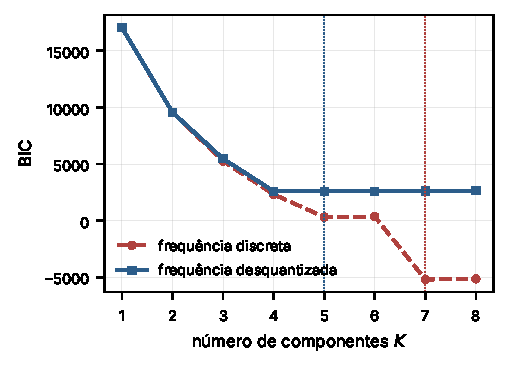
\includegraphics[width=\columnwidth]{figuras/f2_bic.pdf}
\caption{BIC do GMM ($K=1,\dots,8$). Com a frequência discreta, o mínimo cai em $K=7$; com a frequência
desquantizada, em $K=5$, com o platô entre 4 e 6 componentes. A componente extra isola os clientes com
exatamente 2 compras (o piso da variável).}
\label{fig:bic}
\end{figure}

O DBSCAN evidencia a fragilidade da heurística de $\varepsilon$ (Figura~\ref{fig:kdist}). O joelho da
4-distância sugere $\varepsilon=0{,}043$, valor que reflete a densidade dos blocos esporádicos, os mais
densos da base, e com o qual o algoritmo produz 14 grupos e 161 pontos de ruído. Com $\varepsilon=0{,}1$
surgem 5 grupos e 17 ruídos, e a partir de 0,15 os 4 grupos são recuperados, com 2 ruídos nesse valor e
nenhum a partir de 0,2. Assim, a quantidade de ``suspeitos'' rotulados como ruído depende quase
exclusivamente de um parâmetro escolhido por heurística.

\begin{figure}[t]
\centering
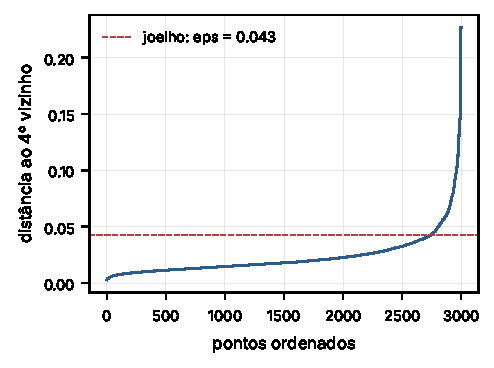
\includegraphics[width=\columnwidth]{figuras/f3_kdist.pdf}
\caption{Curva de 4-distância. O joelho ($\varepsilon=0{,}043$) é dominado pelos blocos mais densos e
fragmenta os demais.}
\label{fig:kdist}
\end{figure}

\begin{table}[t]
\centering\footnotesize
\setlength{\tabcolsep}{1.7pt}
\caption{Comparação das segmentações (silhueta, DB e CH calculados sem os pontos de ruído).
A estabilidade é o ARI médio $\pm$ desvio-padrão em 30 subamostras de 80\%.}
\label{tab:comp}
\begin{tabular}{@{}lccccccc@{}}
\toprule
Método & $K$ & Ruído & Silh. & DB & CH & ARI & Estab. \\
\midrule
\tabinput{tabelas/comparacao.tex}
\bottomrule
\end{tabular}
\end{table}

A Tabela~\ref{tab:comp} sintetiza o ponto central desta primeira parte da argumentação. K-Means, GMM ($K=4$)
e HDBSCAN produziram \emph{a mesma partição}, com métricas idênticas, ARI de 1,000 em relação aos quadrantes
e estabilidade de 1,000. Nesta base, qualquer um dos três pode servir como segmentador, de modo que o
critério de escolha precisa vir de outro lugar.

A Tabela~\ref{tab:perfis} descreve os quatro perfis resultantes. Os clientes \emph{frequentes de ticket alto}
representam 20,3\% da base e respondem por 81,8\% da receita, concentração comum em distribuições de cauda
longa \cite{anderson2004longtail}. Já os \emph{esporádicos de ticket baixo} formam o maior grupo (34,2\%), mas
respondem por apenas 0,9\% da receita.

\begin{table*}[t]
\centering\footnotesize
\caption{Perfis de consumo (partição do GMM com $K=4$; medianas por perfil).}
\label{tab:perfis}
\begin{tabular}{@{}lccccc@{}}
\toprule
Perfil & \begin{tabular}[b]{@{}c@{}}Clientes\\(\%)\end{tabular} & \begin{tabular}[b]{@{}c@{}}Freq.\\mediana\end{tabular} & \begin{tabular}[b]{@{}c@{}}Ticket\\mediano (R\$)\end{tabular} & \begin{tabular}[b]{@{}c@{}}Valor total\\mediano (R\$)\end{tabular} & \begin{tabular}[b]{@{}c@{}}\% da\\receita\end{tabular} \\
\midrule
\tabinput{tabelas/perfis.tex}
\bottomrule
\end{tabular}
\end{table*}

\subsection{Anomalias: os métodos divergem}
\label{sec:anom}
Os scores concordam na ordenação geral, mas divergem justamente no topo, onde se decide o que será revisado. A
correlação de Spearman entre o score GMM e os de K-Means, HDBSCAN e KDE é de 0,942, 0,954 e 0,816,
respectivamente. No top 2\%, contudo, o Jaccard entre GMM e K-Means cai para apenas 0,446, enquanto entre GMM
e HDBSCAN chega a 0,690 e entre GMM e KDE, a 0,600.

\begin{table}[t]
\centering\footnotesize
\setlength{\tabcolsep}{3pt}
\caption{Estabilidade dos scores no top 2\%: Jaccard entre sorteios únicos da desquantização (média
$\pm$ dp, 30 pares) e entre dois ensembles independentes de 30 sorteios. A última coluna é o
Spearman do score com o GMM.}
\label{tab:estab}
\begin{tabular}{@{}lccc@{}}
\toprule
Score & Único & Ensemble & $\rho$ c/ GMM \\
\midrule
\tabinput{tabelas/estab_scores.tex}
\bottomrule
\end{tabular}
\end{table}

Uma única desquantização já altera o ranking (Tabela~\ref{tab:estab}). Nesse cenário, o GMM foi o score mais
estável, com Jaccard de 0,664, seguido de HDBSCAN (0,538), KDE (0,536) e K-Means (0,263). Quando a comparação
é feita entre ensembles de 30 sorteios, o GMM mantém a liderança (0,967), seguido de KDE (0,905), HDBSCAN
(0,875) e K-Means (0,818). Uma explicação provável para a instabilidade do K-Means, que não testamos
diretamente, é o caráter isotrópico da distância euclidiana: ela trata da mesma forma os desvios ao longo do
eixo em que o perfil é naturalmente espalhado e os desvios ao longo do eixo em que ele é estreito.

Os 7 clientes que caem nos vazios entre os blocos, isto é, as anomalias globais, estão \emph{todos} no top 2\%
do GMM, nas posições 6 a 53, e 5 deles aparecem também no top 2\% dos quatro scores. O score contextual,
portanto, não deixa escapar o caso global. A regra ingênua de marcar os 60 maiores gastos totais, por outro
lado, tem apenas 3 clientes em comum com o top 2\% do GMM. Esses três situam-se na borda do perfil frequente
de ticket alto, com 72 compras (a maior frequência da base), 62 compras com ticket de R\$~481,39 e ticket de
R\$~586,51 (o maior do perfil). Foram marcados pela posição que ocupam no perfil, e não pelo valor gasto,
enquanto os demais grandes gastadores são clientes típicos do perfil mais valioso.

Um limiar global sobre o score (top 2\% da base) produz taxas de alerta desiguais entre os perfis: 1,2\% no
esporádico de ticket baixo, 3,2\% no esporádico de ticket alto, 1,7\% no frequente de ticket baixo e 2,5\% no
frequente de ticket alto. Ao adotar um limiar por perfil, fixado no percentil 98 de cada grupo, os alertas
passam a 21, 13, 15 e 13, o que corresponde a cerca de 2\% em cada perfil. Dessa forma, o esforço de revisão
fica proporcional ao tamanho de cada perfil.

\begin{figure}[t]
\centering
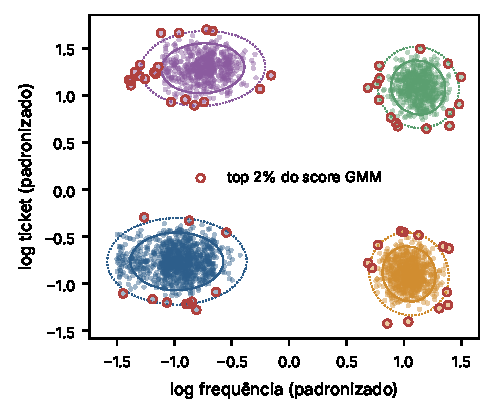
\includegraphics[width=\columnwidth]{figuras/f4_gmm.pdf}
\caption{Componentes do GMM (elipses de 2 e 3 desvios) e os 60 clientes do top 2\% do score
ensemble. Os suspeitos ficam na borda de cada perfil ou nos vazios entre eles.}
\label{fig:gmm}
\end{figure}

A Tabela~\ref{tab:sus} lista os dez maiores scores. Dos 93 clientes que aparecem no top 2\% de pelo menos um
score, 29 estão no top 2\% dos quatro ao mesmo tempo, 22 em três, 16 em dois e 26 em apenas um. Alguns casos
ilustram as hipóteses da Tabela~\ref{tab:fraudes}. O cliente C000657, por exemplo, tem 31 compras com ticket de
R\$~15,52, o menor ticket da base, no perfil frequente de ticket baixo, padrão compatível com \emph{card
testing}. O C000724 fez 2 compras de R\$~719,85 cada; como somente 11 dos 617 clientes do perfil esporádico de
ticket alto têm 2 compras, o caso é compatível com \emph{bust-out} ou com cartão comprometido. O C002556, com 25
compras de R\$~349,98, está no piso de frequência do perfil frequente de ticket alto. Já os clientes C002240 e
C002232, com tickets de R\$~63,12 e R\$~211,32, situam-se dentro do vazio de ticket entre os blocos, o que os
caracteriza como anomalias globais. Essas leituras são \emph{hipóteses de interpretação}, não conclusões: sem
rótulos, nada distingue o C000724 de um cliente que comprou dois eletrodomésticos \cite{bolton2002fraud}.

\begin{table}[t]
\centering\footnotesize
\setlength{\tabcolsep}{2.5pt}
\caption{Top 10 do score GMM (média de 60 desquantizações). ``Cons.'' indica em quantos dos quatro
scores o cliente está no top 2\%.}
\label{tab:sus}
\begin{tabular}{@{}lcclcc@{}}
\toprule
Cliente & Freq. & Ticket & Perfil & Score & Cons. \\
\midrule
\tabinput{tabelas/suspeitos.tex}
\bottomrule
\end{tabular}
\end{table}

\begin{figure}[t]
\centering
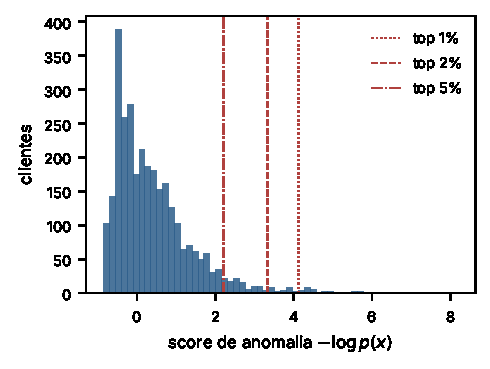
\includegraphics[width=\columnwidth]{figuras/f5_score.pdf}
\caption{Distribuição do score do GMM, com os limiares de top 1\%, 2\% e 5\%. A cauda direita é
longa, sem uma ruptura natural, e por isso o limiar é uma decisão de negócio.}
\label{fig:score}
\end{figure}

\subsection{Por que o GMM: defesa da escolha}
Reunindo as evidências, o GMM é a melhor escolha \emph{para esta base}, por quatro razões que se complementam.
Primeiro, ele entrega a mesma segmentação dos concorrentes (Tabela~\ref{tab:comp}), sem custo de qualidade.
Em segundo lugar, seu score $-\log p(x)$ é contextual por construção, pois a distância de Mahalanobis mede o
desvio na escala e na orientação de cada perfil, o que formaliza a ideia de comparar o cliente com seus pares
\cite{weston2008peer}; além disso, o modelo captou todas as 7 anomalias globais. Em terceiro lugar, foi o score
mais estável, tanto em execução única (0,664) quanto em ensemble (0,967) (Tabela~\ref{tab:estab}). Por fim, por
ser probabilístico, o GMM expõe suas premissas por meio do BIC, que denunciou o efeito da frequência discreta
($K=7$) e, mesmo após a desquantização, apontou o acúmulo no piso de 2 compras ($K=5$). Métodos baseados em
distância e em densidade não oferecem esse tipo de diagnóstico. A escolha final de $K=4$, no entanto, não veio
do BIC, e sim da silhueta, da estabilidade e da interpretabilidade dos perfis.

Os demais candidatos apresentam limitações mais claras. O KDE foi o segundo score mais estável em ensemble
(0,905), mas não segmenta sozinho, depende de uma banda global e apresentou a menor concordância com o GMM
(ρ=0,816). Recomendamos, portanto, usá-lo como score de \emph{confirmação}. Já o DBSCAN e o HDBSCAN rotulam o
ruído de forma binária: o primeiro marcou de 161 pontos a nenhum, conforme o $\varepsilon$ adotado, e o segundo
não marcou nenhum. Nenhum dos dois, portanto, produz uma fila ordenada de revisão.

\subsection{Limitações}
O estudo apresenta limitações que precisam ser explicitadas. Sem rótulos, não é possível medir precisão nem
recall, e a concordância entre métodos não substitui a validação. A base também não tem recência nem informação
temporal, o que deixa tomada de conta e engenharia social fora do alcance da análise (Tabela~\ref{tab:fraudes}).
Além disso, o número de perfis não é inequívoco: o BIC prefere $K=5$ na maioria dos sorteios, e a escolha de
$K=4$, embora justificada, não é automática. O logaritmo amplia diferenças em contagens pequenas, de modo que
parte do score dos clientes com 2 compras decorre dessa escala, e a própria desquantização é heurística. Os
limiares (top 2\% e percentil 98) e os hiperparâmetros são, por fim, escolhas subjetivas. A regularidade dos
blocos, por sua vez, sugere uma base sintética, e a generalização para dados reais não está garantida
\cite{santos2024sintetico}.

% =============================================================================
\section{Conclusões}
Nesta base, quatro perfis bem separados foram recuperados igualmente por K-Means, GMM e HDBSCAN. A escolha do
algoritmo deve, portanto, ser decidida pela qualidade do score de anomalia, e não pela segmentação. O GMM, com
frequência desquantizada e score médio em ensemble, foi o mais estável, captou as anomalias globais e, sobretudo,
identificou os desvios em relação ao perfil que regras de ``valor alto'' deixam passar. Esses resultados sustentam
a tese de que, em dados agregados, a fraude se revela como desvio de perfil, e não como valor extremo.

Para a operadora, a análise sugere alguns encaminhamentos. O score oficial deve ser o $-\log p(x)$ do GMM com
$K=4$, recalculado periodicamente como média de várias desquantizações, e os limiares devem ser definidos por
perfil, no percentil 98 de cada um, de modo que a revisão seja proporcional ao tamanho de cada grupo. A fila de
revisão deve começar pelos 29 clientes em consenso 4/4, seguidos dos 22 em 3/4, enquanto os clientes situados nos
vazios entre os perfis e os que apresentam valores idênticos devem ser investigados à parte, como anomalias
globais e coletivas. Os alertas, por sua vez, podem ser interpretados por perfil: um ticket muito abaixo do
esperado para um perfil de frequência alta sugere a hipótese de \emph{card testing}, ao passo que poucas compras
com ticket no topo do perfil sugerem a de \emph{bust-out}. Como próximo passo, convém registrar o desfecho de cada
revisão, de modo a criar rótulos para treinar um modelo supervisionado, incluir recência e dados temporais e
avaliar Isolation Forest e LOF como referências externas.

\paragraph{Declaração de uso de IA.} Um assistente de IA (Claude, Anthropic) foi usado para apoiar a análise
exploratória, escrever o código dos experimentos, buscar referências e redigir este texto. Todos os números foram
gerados pelo código executado sobre a base, e as referências foram conferidas nas fontes. A responsabilidade pelas
escolhas metodológicas e pelo conteúdo é dos autores.

\bibliographystyle{sbc}
\bibliography{referencias}
\end{document}
